% Inicializa o documento
% define papel, tamanho global de fonte, tipo de documento
\documentclass[a4paper, twoside, 12pt]{article}

	% Pacotes usados
	\usepackage[utf8]{inputenc} % enconding de caracteres
	\usepackage[brazil]{babel}  % locale pt_BR
	\usepackage[lmargin=2cm, rmargin=2cm, tmargin=2cm, bmargin=2cm]{geometry} % margens da folha
	\usepackage{indentfirst} % sempre indenta o primeiro parágrafo

	% Matemática	
	\usepackage{amsmath}
	\usepackage{amsfonts}
	\usepackage{gensymb}
	
	% Para links e url
%	\usepackage[hidelinks]{hyperref}
	
	\usepackage{listings} % listagem de código-fonte
	\renewcommand*{\lstlistingname}{Listagem} % texto para listagem de código
	\usepackage{color} % cor para usar na listagem de código-fonte
%	\usepackage{svg}
	\usepackage{graphicx,xcolor} % para inserir imagens
	\usepackage[nottoc,notlot,notlof]{tocbibind} % adiciona o tópico Referências ao Sumário
	\usepackage{textcomp} % accesso \textquotesingle

	% Para desenhar grafos
	\usepackage{tikz}
	\usetikzlibrary{arrows,positioning,shapes,decorations}

	% Desenhar circulos
%	\usepackage{tkz-euclide}
%	\usetkzobj{all}

	% Escrever algoritmos em pseudo-código
%	\usepackage[portuguese,linesnumbered]{algorithm2e}

	% Tabelas
	\usepackage{booktabs}
	\usepackage{caption}

	% Estilos para usar nos grafos
	\tikzset{
		>=stealth',
		punkt/.style={
			rectangle,
			text centered,
			inner sep=0.7em,
			draw,
			fill=blue!5
		},
		pil/.style={
			->,
			thick,
			shorten <=2pt,
			shorten >=2pt
		}
	}

	% Para plotar gráficos
%	\usepackage{pgfplots}
%	\pgfplotsset{width=10cm,compat=1.9}

	% Define cores para o highlight de código-fonte
	\definecolor{dkgreen}{rgb}{0,0.6,0}
	\definecolor{gray}{rgb}{0.5,0.5,0.5}
	\definecolor{mauve}{rgb}{0.58,0,0.82}
	
	% Define configuração para listagem de código-fonte em linguagem C
	\lstset{
		frame=tb,
		language=C,
		aboveskip=2mm,
		belowskip=2mm,
		showstringspaces=false,
		columns=flexible,
		basicstyle={\small\ttfamily},
		numbers=none,
		keywordstyle=\color{blue},
		commentstyle=\color{dkgreen},
		stringstyle=\color{mauve},
		breaklines=true,
		breakatwhitespace=false,
		tabsize=4
	}

% Começo do documento
\begin{document}

	% Define algum espaçamento que eu não lembro, hehe :)
	\setlength\parskip{0.3cm}

	% Insere a Capa
	% Começo da folha de Capa
\begin{titlepage}

		% Título
		\title{
\textsc {\large Universidade de São Paulo\\
Instituto de Ciências Matemáticas e de Computação}\\[1cm]
{\large SSC0143 -- Programação Concorrente}\\[5cm]
{\LARGE Trabalho 1 -- Cálculo do $\pi$} e Black-Scholes\\[4cm]
		}

		% Autores
		\author{
Elias Italiano Rodrigues -- 7987251\\
Rodolfo Megiato de Lima -- 7987286\\
Vinicius Katata Biondo -- 6783972
		}

		% Inserção manual de data
		\date{
\vfill São Carlos, 5 de setembro de 2014
		}


		% Cria a Capa
		\maketitle
\texttt{Repositório: https://code.google.com/p/pc2014-02-grupo2-turmab/}
		\thispagestyle{empty}

% Fim da folha de Capa
\end{titlepage}

	
	% Reseta contador de página para 1 (assim não conta a Capa como página)
	\setcounter{page}{1}
	
	% Insere as outras partes do documento
	% Cria o Sumário
\tableofcontents

% Cria uma nova página, forçando o Sumário a ficar numa página separada
\newpage


	\section{Introdução \label{sec:introducao}}

\subsection{\textbf{NP}-\textit{completo}}

Como visto na disciplina de Teoria da Computação e Linguagens Formais, não é possível resolver a grande maioria dos problemas em computação, ou porque são indecidíveis ou porque não se conhece algoritmo capaz de resolvê-los em tempo polinomial. Geralmente, consideramos os problemas que são resolvidos por algoritmos de tempo polinomial como tratáveis, ou fáceis, e os demais problemas que requerem tempo super-polinomial como intratáveis, ou difíceis.

Na classe de problemas \textbf{NP}-\textit{completo} estão os problemas para os quais ainda não foi descoberto um algoritmo de tempo polinomial que os resolva, nem ainda alguém conseguiu provar que um algoritmo de tempo polinomial pode existir para algum desses problemas. A questão ``$\mathbf{P} = \mathbf{NP}$?'' é justamente sobre essa última afirmação e tem sido uma das questões abertas mais perplexas da Teoria da Computação desde que foi proposta em 1971.

Considerando que $\mathbf{P} \neq \mathbf{NP}$, o diagrama da Figura~\ref{fig:np} representa onde se encontram os problemas da classe \textbf{NP}-\textit{completo}.

\begin{figure}[h]
	\centering
	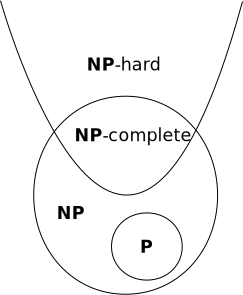
\includegraphics[scale=0.8]{./input/np.pdf}
	\caption{Diagrama das classes de problemas. \label{fig:np}}
\end{figure}

\subsection{Objetivo}

Este trabalho, dentro dos tópicos de Classes de Complexidade (\textit{Complexity Classes}) da disciplina de Linguagens Formais e Teoria da Computação, consiste em explicar do que se trata o Problema da Soma dos Subconjuntos (\textit{Subset Sum Problem}) e apresentar uma prova de sua \textbf{NP}-\textit{completude}. Por ser um problema conhecido e já estudado, este trabalho é um \textbf{exercício de pesquisa} em que são consultadas referências na literatura e sintetizadas aqui pelo grupo.

Todo material pesquisado para este trabalho encontra-se nos capítulos 34 e 35 do livro \textit{Introduction to Algorithms}~\cite{bib:cormen} sugerido como referência nos \textit{slides} de aula da disciplina.

% inkscape -D -z --file=./input/smooth.svg --export-pdf=./input/smooth.pdf


	\section{Como ocorre a espionagem? \label{sec:como-ocorre}}

Os motivos que levam a atividade de espionagem computacional são vários. Uns dos mais comuns são quando existe algum tipo de suspeita sobre ações de uma pessoa nos sistemas de TI de uma empresa ou instituição; espionagem para obter informações de vantagem competitiva; para testes de segurança; ou simplesmente por diversão/curiosidade.

	\section{Quais são as implicações? \label{sec:implicacoes}}

\subsection{Criptografia \label{sec:criptografia}}

Atualmente, com o advento do protocolo HTTPS, conhecido como o protocolo HTTP seguro, os ataques de \textit{sniffing} são prevenidos, pois todas as informações das mensagens são criptografadas, dificultando muito a interpretação desses dados pelo atacante. Esse protocolo foi construído com o objetivo de prevenir esses tipos de ataques.

Assim, com o HTTPS, as mensagens não podem ser mais lidas por meio do ataque de \textit{sniffing}, mas ainda é possível obter informações sobre remetente e o destinatário. Ainda assim, pode-se também realizar ataques \textit{man-in-the-middle} e de \textit{replay}, já que ainda há a captura do pacote.

Ataque \textit{man-in-the-middle} é uma forma de ataque em que os dados trocados entre duas partes, por exemplo você e o seu banco, são de alguma forma interceptados, registrados e possivelmente alterados pelo atacante sem que as vítimas percebam. O atacante pode decidir retransmitir entre os legítimos participantes os dados inalterados, com alterações ou bloquear partes da informação. Já ataques de \textit{replay} é uma outra forma de ataque onde o interceptador reproduz as mensagens interceptadas sem alterar o conteúdo.

\subsection{Leis \label{sec:leis}}

Com relação as atividades de interceptações de comunicações de informática, no Brasil vigora a Lei Nº 9.296, de 24 de Julho de 1996 que segundo o artigo 10: ``Constitui crime realizar interceptação de comunicações telefônicas, de informática ou telemática, ou quebrar segredo da Justiça, sem autorização judicial ou com objetivos não autorizados em lei."~\cite{bib:lei1}

Nos Estados Unidos, também existe uma lei para privacidade de comunicações eletrônicas  de 1986 que diz ser ilegal intencionalmente, ou propositadamente interceptar, divulgar ou usar o conteúdo de qualquer comunicação por fio, oral ou eletrônica através de o uso de um dispositivo de escuta.~\cite{bib:lei2}

\subsection{Caso \label{sec:caso}}

Segundo uma notícia publicada em 2011, o Google poderia ser investigado por interceptar, sem autorização judicial, dados privados de redes sem fio brasileiras. Segundo o pesquisador cearense Pablo Ximenes, professor de Ciência da Computação e pesquisador do Information Security Research Team (Insert), as interceptações aconteceram entre 2009 e 2010, durante o levantamento de dados para o Google Street View.~\cite{bib:caso}

Segundo Ximenes, as interceptações ilegais aconteceram por meio do sistema de coleta de dados de redes sem fio realizada pelo veículo autônomo da Google. Ele afirma que o veículo usou uma técnica de captura de dados conhecida como \textit{sniffing}. Com ela, todas as ondas de rádio destinadas a uma rede sem fio eram interceptadas pela empresa. Isso inclui dados privados de usuários, como fotos, senhas, emails e documentos pessoais.

Em estudo realizado pelo Insert, foi constatado que o serviço da Google teria interceptado aproximadamente 4.300 redes sem fio apenas em Minas Gerais. Segundo Jairo Ponte, advogado e professor de Direito da Faculdade Cearense (FaC) a Google teria infrigido a lei federal 9.296/96, conhecida como Lei da Interceptação Telefônica, segundo o artigo 10.

Respondendo a acusação, a empresa admitiu que seu veículo interceptou redes sem fio, mas alegou só ter acessado redes públicas. Segundo a Google, os veículos capturaram apenas sinais do tipo \textit{beacon}, mensagens públicas das redes sem fio. Em nova investigação, os pesquisadores desmentiram as declarações, ao provarem que a empresa também acessou \textit{payloads}.

Para tentar resolver o impasse, o próprio Google encomendou uma análise de códigos e programas utilizados pelo Street View. O estudo confirmou as denúncias, provando que o veículo coletou dados de conexões sem fio. Na lista apresentada pela análise, estavam emails completos, páginas web e senhas.

O Google justificou o fato, afirmando que as interceptações ocorreram de forma não-intencional. Segundo a empresa, tudo não passou de erro de programação dos engenheiros do Street View. Além disso, o Google alegou que apenas acessou informações incompletas, já que o veículo estava em movimento.

Pablo Ximenes afirma que as interceptações foram feitas de forma intencional. Um indício seria o registro da patente ``aproximação de localização baseada em redes sem fio", proposta pelo Google em 2008 e registrada em janeiro de 2010. Entre outros, a patente descreve o mesmo mecanismo de captura de dados presente no veículo do Street View.

Para Ximenes, a ideia de que um erro no código de captura tenha passado despercebido é ``no mínimo ingênua". ``As rotinas de teste do Google estão entre as mais rigorosas do mundo. Se fosse um erro por parte dos engenheiros, duvido que ele não fosse sido resolvido ainda nos estágios de teste", ponderou o pesquisador.

Como consequência das pressões, o Google suspendeu a coleta de dados de redes sem fio nos carros do Street View. Essa medida continua em vigor até hoje. Apesar disso, ainda existe debate sobre quais foram as reais proporções das interceptações promovidas pelo serviço.

	\chapter{Conclusão}
\label{ch:conclusao}

É inquestionável que para aumentar a escalabilidade da blockchain são necessárias mudanças no protocolo. Aprimoramentos tecnológicos somente não são suficientes para escalar o sistema. Por isso, modificações como o aumento do tamanho máximo do bloco são necessárias juntamente com outras inovações no protocolo.

Considerando os pensamentos da Escola Austríaca de economia, o livre mercado por enquanto é o arranjo que melhor define os preços de produtos e serviços e cria incentivos desfavoráveis à corrupção. Logo, um livre mercado é preferível a um planejamento central. O autor deste documento defende que este mesmo pensamento aplicado ao tamanho máximo do bloco resulta em melhores blocos e, quando somado às propostas da SegWit e Lightning Network, resulta em uma melhor escalabilidade para o Bitcoin.

O projeto de criptomoeda é intrinsecamente uma proposta de um livre mercado de moedas, pois permite a livre concorrência entre elas. E, por dentro de uma criptomoeda, devido ao seu mecanismo de consenso e ao seu código-fonte aberto, mudanças nos protocolos também estão suscetíveis a um livre mercado. Com isso, conclui-se que Bitcoin \textbf{é}  Unlimited. Isso ainda não é evidente, pois existe uma carência de profissionais capacitados para propor e implementar mudanças nos softwares (lembrando que Bitcoin é um software crítico). Conforme a oferta de profissionais capacitados na área aumentar, essa relação se tornará mais evidente.

No entanto, observa-se na comunidade do Bitcoin pessoas que, apesar de parecerem favoráveis ao livre mercado, propõem técnicas de intervencionismo para controlar o tamanho do bloco. Em um livre mercado de tamanhos máximos de blocos e taxas de transação, a tendência é que os valores convirjam para aqueles que melhor valorizam a criptomoeda e não prejudicam a rede. Outra preocupação é com o perigo de centralização da rede causado pela concentração do poder de \textit{hash} em poucos mineradores/\textit{pools}. Tal centralização não ocorreria em um ambiente livre, pois um minerador que busca pelo maior lucro limitaria seu poder de \textit{hash} para não tomar grande parte da rede. Caso o contrário, ele estaria contribuindo para seu próprio prejuízo, uma vez que, havendo notória centralização, a moeda seria desvalorada pelas demais entidades da rede --- desenvolvedores, usuários e \textit{stakeholders} --- que migrariam para uma criptomoeda concorrente.

Então, como passo gradual, pode-se adotar o Classic e, posteriormente, a migração para o Unlimited com alterações no protocolo para suportar SegWit e Lightning Network.

Ainda assim, toda hesitação quanto ao rumo do projeto Bitcoin é bastante compreensível, visto que más decisões podem causar grandes prejuízos às entidades envolvidas e, de modo geral, criptomoeda ainda é uma tecnologia nova e em constante debate e desenvolvimento. Ademais, não tão cedo altcoins conseguirão competir ao mesmo nível com o Bitcoin, uma vez que a maioria dos investimentos e dos desenvolvedores experientes estão focados nele. Espera-se por grandes mudanças nas próximas décadas e inovações no uso de blockchains como visionado pela Ethereum.

\section{Contribuições}

Este trabalho reúne e comenta sobre assuntos relacionados a área de Criptomoeda e serve para introduzir pessoas interessadas ao tema e ao problema atual de escalabilidade da blockchain por meio de algumas propostas. Além dos profissionais altamente experientes que investem em projetos de criptomoeda, espera-se que a pesquisa sobre criptomoedas no âmbito acadêmico, que aliás ainda é pequena no Brasil, cresça nos próximos anos e possa fortalecer a tecnologia com apoio da academia.

Pesquisar para este trabalho proporcionou bons momentos de estudos sobre tecnologias interessantes e com um evidente potencial disruptivo, podendo causar grandes mudanças sociais, assim como fez o surgimento da Internet.

\section{Trabalhos Futuros}

Aprofundado o conhecimento no protocolo e na arquitetura do Bitcoin, pode-se no futuro estagiar na área com desenvolvimento de aplicações ou aprofundar-se na pesquisa com simulações sobre as propostas de escalabilidade, ou estudos sobre a segurança da rede Bitcoin e criptografia ou ainda estudar o código-fonte e contribuir para o projeto.

	\newpage

% Começo das Referências
%\begin{thebibliography}{9}

% Fim das Referências
%\end{thebibliography}


% Fim do documento
\end{document}
